\section{Markov-Ketten, Hidden Markov Modelle}
Eine Markov-Kette ist ein stochastischer Prozess, der durch Zustände und Über-gangswahrscheinlichkeiten beschrieben wird.
\begin{figure}[htbp]
	\centering
		\begin{tikzpicture}[node distance=2cm]
			\node[state] (z_0)                {$z_0$};
			\node[state] (z_1) [right of=z_0] {$z_1$};
			\path[->] 
				(z_0) 
					edge [loop above] node {0,3} ()
					edge [bend left, above] node {0,7} (z_1)
				(z_1) 
					edge [loop above] node {0,6} ()
					edge [bend left, below] node {0,4} (z_0);
		\end{tikzpicture}
\end{figure}

Damit lassen sich modellieren:
\begin{itemize}
	\item Texte in natürlicher Sprache (Zustände: Buchstaben)
	\item DNA-Sequenzen (Zustände: A,C,G,T)
	\item Navigation im Internet (Zustände: Webseiten)
\end{itemize}


\subsection{Hidden Markov Model (HMM)}
\begin{shaded}
  \noindent
  \textbf{Def.:} Ein HHM ist eine Markov-Kette, die in jeden Zustand z ein Zeichen a ausgibt mit der Wahrscheinlichkeit \(q_z(a)\).
\end{shaded}
\begin{figure}[htbp]
	\centering
	\begin{tikzpicture}[node distance=4cm]
		\node[state] (z_0)                {\(z_0\)};
		\node[state] (z_1) [right=4cm of z_0] {\(z_1\)};
		\node[emission] (a) [below of=z_0] {a};
		\node[emission] (b) [below of=z_1] {b};
		\path[->] 
			(z_0) 
				edge [loop above] node {0,5} ()
				edge [bend left, above] node {0,5} (z_1)
				edge [left] node {0,6} (a)
				edge [left] node {0,4} (b)
			(z_1) 
				edge [loop above] node {0,9} ()
				edge [ above] node {0,1} (z_0)
				edge [right] node {0,9} (b)
				edge [right] node {0,1} (a);
	\end{tikzpicture}
\end{figure}
Beobachtet werden nur die vom HMM ausgegebenen Zeichen.
Unbekannt ist die Zustandsfolge.
Mit HMM können modelliert werden z.B.:
\begin{itemize}
	\item Codierende Regionen in DNA\\
		Zustände: A,C,T,G in codierenden und nicht codierenden Regionen\\
		Ausgegebene Zeichen: Jeweils A,C,T,G
	\item Nachrichtenübertragung\\
		Markov-Kette, die Texte modelliert\\
		In einem Zustand z wird das Zeichen z ausgegeben mit großer Wahrscheinlichkeit (z.B. 0,95), andere Zeichen mit geringer W'keit.
	\item Spracherkennung\\
		Vorgehen: Audio-Signal $\to$ FFT $\to$ Phoneme $\to$ Wort\\
		Zustände: Phoneme, die der Sprecher gesprochen hat.\\
		Ausgegebenen Zeichen: Phoneme, die das System erkannt hat oder das vom System erkannte Wort.
\end{itemize}

\subsubsection{Mathematische Behandlung}
Sei \(Z_k\) eine Zufallsvariable, die den Zustand des HMM im Schritt \(k\) angibt.
Aus \(Z_1\) ergibt sich die Startverteilung \[\pi_k=P(Z_1=k)\] der Markov-Kette.
Da \(Z_{k+1}\) nur von \(Z_k\) abhängt, folgt:
\begin{eqnarray*}
	&&P(\underbrace{Z_{k+1}}_{\text{Zufallsvariable}}=\underbrace{Z_{i_{k+1}}}_{\text{Zustand}}
    \mid Z_k =z_{i_k}, \ldots, Z_1=z_{i_1})\\
	&=& P(Z_{k+1} = z_{i_{k+1}}\mid Z_k=z_{i_k})\\
	&=:& p(Z_{i_k},Z_{i_{k+1}})
\end{eqnarray*}
Sei \(A_k\) die Zufallsvariable, die das in Schritt \(k\) ausgegebene Zeichen angibt.
\(A_k\) hängt nur von \(Z_k\) ab:
\[P(A_k=a\mid Z_k=z_{i_k}, \ldots, Z_1=z_1) = P(A_k=a\mid Z_k=z_{i_k}) := q_{z_{i_k}}(a)\]
Die charakteristischen Größen eines HMM sind damit \(\pi_k,\; p(z,z'),\; q_z(a)\).

\subsubsection{Rekonstruktion der Zustandsfolge}
Für eine Folge \(a_1,\dots,a_n\) von beobachteten Zeichen suchen wir eine Folge \(z_{i_1}, \ldots, z_{i_n}\) von Zuständen, so dass
\[P(Z_1=z_{i_1}, \ldots, Z_n=z_{i_n} \mid  A_1=a_1, \ldots, A_n=a_n)\]
maximal ist.
Da in
\begin{eqnarray*}
    \frac{P(Z_1=z_{i_1}, \dots, Z_n=z_{i_n},\; A_1 = a_1, \dots, A_n=a_n)}{P(A_1=a_1, \dots, A_n=a_n)} \\
\end{eqnarray*}
der Nenner unabhängig von der Lösung ist (da er der Beobachtung entspricht), maximieren wir den Zähler.
%\begin{eqnarray*}
	%&&P(Z_1=z_1, \dots, Z_n=z_n \mid  A_1=a_1, \dots A_n=a_n)\\
	%&=& \frac{P(Z_1=z_1, \dots, Z_n=z_n) \cap P(A_1 = a_1, \dots, A_n=a_n)}{P(A_1=a_1, \dots, A_n=a_n)} \\
	%&=& \frac{P(Z_1=z_1, \dots, Z_n=z_n, A_1 = a_1, \dots, A_n=a_n)}{P(A_1=a_1, \dots, A_n=a_n)}
%\end{eqnarray*}

Sei
\begin{eqnarray*}
	t(z_{i_n},n) &=& P(Z_1=z_{i_1}, \dots, Z_n=z_{i_n}, A_1=a_1, \dots, A_n=a_n)\\
		&=& P(A_n=a_n\mid Z_1=z_{i_1}, \dots, Z_n=z_{i_n}, A_1=a_1, \dots, A_{n-1} = a_{n-1}) \cdot \\
		&& P(Z_1=z_{i_1}, \dots, Z_n=z_{i_n}, A_1=a_1, \dots, A_{n-1}=a_{n-1})\\
		&=& P(A_n=a_n\mid Z_n=z_{i_n}) \cdot \\
		&& P(Z_1=z_{i_1}, \dots, Z_n=z_{i_n}, A_1=a_1, \dots, A_{n-1}=a_{n-1})\\
		&=& q_{z_{i_n}}(a_n) \cdot\\
		&& P(Z_n=z_{i_n}\mid Z_1=z_{i_1}, \dots, Z_{n-1}=z_{i_{n-1}}, A_1=a_1, \dots, A_{n-1}=a_{n-1}) \cdot\\
		&& P(Z_1=z_{i_1},\dots, Z_{n-1}=z_{i_{n-1}}, A_1=a_1, \dots, A_{n-1}=a_{n-1})\\
		&=& q_{z_{i_n}}(a_n) \cdot P(Z_n=z_{i_n}\mid Z_{n-1}=z_{i_{n-1}}) \cdot \\
		&& P(Z_1=z_{i_1}, \dots, Z_{n-1}=z_{i_{n-1}}, A_1=a_1, \dots, A_{n-1}=a_{n-1})\\
		&=& q_{z_{i_n}}(a_n) \cdot p(z_{i_{n-1}},z_{i_n}) \cdot t(z_{i_{n-1}},n-1)
\end{eqnarray*}



\subsection{Viterbi-Algorithmus}
Der Viterbi-Algorithmus ist ein Algorithmus der dynamischen Programmierung zur Bestimmung der wahrscheinlichsten Sequenz
von verborgenen Zuständen bei einem gegebenen Hidden Markov Model (HMM) und einer beobachteten Sequenz von Symbolen.
Diese Zustandssequenz wird auch als Viterbi-Pfad bezeichnet.
\[
    t(Z,n) =
    \begin{cases}
        q_Z(a_1) \cdot \pi_Z 								& \text{für } n=1\\
        q_Z(a_n) \cdot \displaystyle \max_{z'}\left(p(z',z) \cdot t(z',n-1)\right) & \text{für } n>1\\
    \end{cases}
\]
Die Laufzeit beträgt \(\underbrace{\mathcal{O}(|Z| \cdot n)}_{\text{Größe der Tabelle}} \cdot \underbrace{\mathcal{O}(|Z|)}_{\text{Aufwand pro Zelle}} = \mathcal{O}(|Z|^2 \cdot n)\)
\begin{figure}[htbp]
	\centering
	\begin{tikzpicture}[node distance=1.5cm]
		\node[state] (z)                  {z};
		\node[state] (z') [left=1.5cm of z]     {z'};
		\node[state] (e1) [above of=z']  {};
		\node[state] (e2) [below of=z'] {};
		\node (a) [below=.5cm of e2] {\(\underbrace{a_1\; \dots\; a_{k-1}}_{t(z',k-1)}\)};
		\node[emission] (ak) [below of=z] {$a_k$};
		\path[->] 
			(e1) edge (z)
			(e2) edge (z)
			(z') edge [above] node {P(z',z)} (z)
			(z)	 edge [right] node {\(q_z(a_k)\)} (ak);
	\end{tikzpicture}
    \caption{Verdeutlichung des Viterbi-Algorithmusses.}
    \label{fig:viterbi}
\end{figure}

Um die numerische Stabilität des Verfahrens zu erhöhen, kann man mit Logarithmen der Werte rechnen.

\subsubsection{Beispiel}
Gegeben sei das HMM-Model in Abbildung \ref{fig:hmmbsp} mit der Folge ``k z z k k z k k k k k k'' (mit k=Kopf, z=Zahl).
Berechnen Sie die wahrscheinlichste Zustandsfolge die diese Folge erzeugt hat
\begin{figure}[htbp]
	\centering
	\begin{tikzpicture}[node distance=2cm]
		\node[state] (z0)                 {z0};
		\node[state] (z1) [right of=z0]   {z1};
		\node[emission] (k) [below of=z0] {k};
		\node[emission] (z) [below of=z1] {z};
		\path[->] 
			(0.9,1.5) 
				edge [left] node {0,9} (z0)
				edge [right] node {0,1} (z1)
			(z0) 
				edge [loop left] node {0,9} ()
				edge [bend left, above] node {0,1} (z1)
				edge [left] node {0,5} (k)
				edge [left] node {0,5} (z)
			(z1) 
				edge [loop right] node {0,9} ()
				edge [bend left, above] node {0,1} (z0)
				edge [right] node {0,1} (z)
				edge [right] node {0,9} (k);
	\end{tikzpicture}
    \caption{HMM für Beispiel X.}
    \label{fig:hmmbsp}
\end{figure}

\begin{center}
\begin{tabular}{cccc}
				& \(z_{0}\) & \(z_{1}\) & \\ \hline
\(t(z',1)\)= k	& \(0,5\cdot0,9 = 0,4500;\) & \(0,9\cdot0,1 = 0,0900\) & \(z_{0}\) \\ \hline
\(t(z',2)\)= z	& \(	\begin{array} {r@{}l@{}}
							0,5\cdot\max\{	& 0,9\cdot0,45; \\
											& 0,1\cdot0,09\}\\
										   =& 0,2025
					\end{array}
					\)
				&  \(	\begin{array} {r@{}l@{}}
							0,1\cdot\max\{	& 0,9\cdot0,09; \\
											& 0,1\cdot0,45\}\\
										   =& 0,0081
					\end{array}
					\) & \(z_{0}\) \\ \hline
\(t(z',3)\)= z	& \(	\begin{array} {r@{}l@{}}
							0,5\cdot\max\{	& 0,9\cdot0,2; \\
											& 0,1\cdot0,0081\}\\
										   =& 0,091125
					\end{array}
					\)
				&   \(	\begin{array} {r@{}l@{}}
							0,1\cdot\max\{	& 0,9\cdot0,008; \\
											& 0,1\cdot0,2\}\\
										   =& 0,002025
					\end{array}
					\) & \(z_{0}\)\\ \hline
\(t(z',4)\)= k	& \(	\begin{array} {r@{}l@{}}
							0,5\cdot\max\{	& 0,9\cdot0,09; \\
											& 0,1\cdot0,002\}\\
										   =& 0,04100625
					\end{array}
					\)
				&   \(	\begin{array} {r@{}l@{}}
							0,9\cdot\max\{	& 0,9\cdot0,002; \\
											& 0,1\cdot0,09\}\\
										   =& 0,00820125
					\end{array}
					\) & \(z_{0}\)\\ \hline
\(t(z',5)\)= k	& \(	\begin{array} {r@{}l@{}}
							0,5\cdot\max\{	& 0,9\cdot0,041; \\
											& 0,1\cdot0,0082\}\\
										   =& 0,0184528125
					\end{array}
					\)
				&   \(	\begin{array} {r@{}l@{}}
							0,9\cdot\max\{	& 0,9\cdot0,0082; \\
											& 0,1\cdot0,041\}\\
										   =& 0,0066430125
					\end{array}
					\) & \(z_{0}\)\\ \hline
\(t(z',6)\)= z	& \(	\begin{array} {r@{}l@{}}
							0,5\cdot\max\{	& 0,9\cdot0,018; \\
											& 0,1\cdot0,007\}\\
										   =& 0,0083037656
					\end{array}
					\)
				&   \(	\begin{array} {r@{}l@{}}
							0,1\cdot\max\{	& 0,9\cdot0,007; \\
											& 0,1\cdot0,018\}\\
										   =& 0,00063
					\end{array}
					\) & \(z_{0}\)\\ \hline
\(t(z',7)\)= k	& \(	\begin{array} {r@{}l@{}}
							0,5\cdot\max\{	& 0,9\cdot0,0081; \\
											& 0,1\cdot0,00063\}\\
										   =& 0,0037366945
					\end{array}
					\)
				&   \(	\begin{array} {r@{}l@{}}
							0,9\cdot\max\{	& 0,9\cdot0,00063; \\
											& 0,1\cdot0,0083\}\\
										   =& 0,0007473389
					\end{array}
					\) & \(z_{1}\)\\ \hline
\(t(z',8)\)= k	& \(	\begin{array} {r@{}l@{}}
							0,5\cdot\max\{	& 0,9\cdot0,0037; \\
											& 0,1\cdot0,00075\}\\
										   =& 0,0016815254
					\end{array}
					\)
				&   \(	\begin{array} {r@{}l@{}}
							0,9\cdot\max\{	& 0,9\cdot0,00075; \\
											& 0,1\cdot0,0037\}\\
										   =& 0,0006053445
					\end{array}
					\) & \(z_{1}\)\\ \hline
\(t(z',9)\)= k	& \(	\begin{array} {r@{}l@{}}
							0,5\cdot\max\{	& 0,9\cdot0,00162; \\
											& 0,1\cdot0,00059\}\\
										   =& 0,0007566806
					\end{array}
					\)
				&   \(	\begin{array} {r@{}l@{}}
							0,9\cdot\max\{	& 0,9\cdot0,0006; \\
											& 0,1\cdot0,00162\}\\
										   =& 0,0004903291
					\end{array}
					\) & \(z_{1}\)\\ \hline
\(t(z',10)\)= k	& \(	\begin{array} {r@{}l@{}}
							0,5\cdot\max\{	& 0,9\cdot0,000729; \\
											& 0,1\cdot0,0004779\}\\
										   =& 0,000328
					\end{array}
					\)
				&   \(	\begin{array} {r@{}l@{}}
							0,9\cdot\max\{	& 0,9\cdot0,0004779; \\
											& 0,1\cdot0,000729\}\\
										   =& 0,0003971665
					\end{array}
					\) & \(z_{1}\)\\ \hline
\(t(z',11)\)= k	& \(	\begin{array} {r@{}l@{}}
							0,5\cdot\max\{	& 0,9\cdot0,000328; \\
											& 0,1\cdot0,0006561\}\\
										   =& 0,0001476
					\end{array}
					\)
				&   \(	\begin{array} {r@{}l@{}}
							0,9\cdot\max\{	& 0,9\cdot0,0006561; \\
											& 0,1\cdot0,000328\}\\
										   =& 0,0005314
					\end{array}
					\) & \(z_{1}\)\\ \hline
\(t(z',12)\)= k	& \(	\begin{array} {r@{}l@{}}
							0,5\cdot\max\{	& 0,9\cdot0,0001476; \\
											& 0,1\cdot0,0005314\}\\
										   =& 0,00006642
					\end{array}
					\)
				&   \(	\begin{array} {r@{}l@{}}
							0,9\cdot\max\{	& 0,9\cdot0,0005314; \\
											& 0,1\cdot0,001476\}\\
										   =& 0,0004304
					\end{array}
					\) & \(z_{1}\)
\end{tabular}
\end{center}
Damit ergibt sich die Zustandsfolge \(z_{0} \rightarrow z_{0} \rightarrow z_{0} \rightarrow z_{0} \rightarrow z_{1} \rightarrow z_{1}\rightarrow z_{1} \rightarrow z_{1}\rightarrow z_{1}\rightarrow z_{1}\)

Ausgehend vom maximum des letzten Zustandes ist der Vorgänger der Zustand, aus dem das Maximum hervorging.

\subsection{Parameterschätzung}
Die Parameter eines HMM sind Startverteilung, Übergangs- und Emissionswahrscheinlichkeiten.
Gegeben sei eine Menge von Trainingssequenzen.

\subsubsection{Überwachtes Lernen}
Wenn für alle Trainingssequenzen die Zustandsfolge bekannt ist, lassen sich ML-Schät"-zer (Maximum-Likelihood) für alle Parameter angeben.
Entsprechende Trainingssequenzen lassen sich häufig erzeugen, z.B.
\begin{itemize}
	\item Nachrichtenübertragung: Nachricht mehrfach senden und empfangen.
	\item Sprachverarbeitung: Beispielsätze für die darin enthaltenen Phoneme bekannt sind, werden vorgelesen.
\end{itemize}
Seien \(z,z\)' Zustände des HMM und \(h(z,z')\) die Häufigkeit des Übergangs von \(z\) nach \(z'\) in den Trainingssequenzen.
Sei ferner \(h_0(z)\) die Häufigkeit von \(z\) als Startzustand.
Da der Übergang von \(z\) nach \(z\)' durch eine Bernoulli-Verteilung beschrieben werden kann, sind
\[
	\hat{p}(z,z')=\frac{h(z,z')}{\sum\limits_{z''} h(z,z'')} \qquad
	\hat\pi_z=\frac{h_0(z)}{\|Z\|}
\]
ML-Schätzer für \(p(z,z')\) bzw \(\pi_z\).
Entsprechend ist
\[
	\hat{q}_z(a)=\frac{h_z(a)}{\sum\limits_{a'} h_z(a')}
\]
ein ML-Schätzer für \(q_z(a)\), wobei \(h_z(a)\) die Häufigkeit der Emission des Zeichens \(a\) im Zustand \(z\) in den Trainingssequenzen ist.
Wenn im HMM gilt: \(\sum_a q_z(a)=1\), ist \(\sum_{a'} h_z(a')\) die Summe der Längen aller Trainingssequenzen.

\subsubsection{Unüberwachtes Lernen}
Wenn die Zustandsfolge für die Trainingssequenzen nicht bekannt ist, können die unbekannten Parameter durch ein iteratives Verfahren geschätzt werden.
Idee dazu:
\begin{itemize}
	\item Mit zufälligen Parametern beginnen oder alle Wahrscheinlichkeiten gleich setzen.
	\item Aus den Trainingssequenzen mit dem Viterbi-Algorithmus die Zustandsfolge rekonstruieren, damit die Schätzwerte für \(h_0(z),\; h(z,z'),\; h_z(a)\) berechnen.
	\item Mit den oben beschriebenen Verfahren Schätzer für die Parameter des HMM berechnen.
\end{itemize}
Die letzten beiden Schritte werden wiederholt, bis ein Terminierungskriterium erreicht wird.

\subsubsection{Viterbi-Training}
\begin{algorithm}
	\begin{algorithmic}[1]
		\State {Parameter \(p(z,z'),\; \pi_z,\; q_z(a)\) zufällig oder durch überwachtes Lernen initialisieren.}
		\Repeat
		\State{Wende den Viterbi-Algorithmus auf die Trainingssequenzen an}
		\State{Berechne \(\hat{p}(z,z'),\; \hat\pi_z,\; \hat{q_z}(a)\)}
		\Until{keine Änderung an \(\hat{p}(z,z'),\; \hat\pi_z,\; \hat{q_z}(a)\).}
	\end{algorithmic}
	\caption{Unüberwachtes Lernen für HMM.}
	\label{alg:hmmus}
\end{algorithm}
Der Algorithmus \ref{alg:hmmus} terminiert, weil schließlich der Viterbi-Algorithmus stets die gleiche Folge liefert (ohne Beweis) und die geschätzten Parameter sich daher nicht mehr ändern.
Das Viterbi-Training liefert jedoch keinen ML-Schätzer für die unbekannten Parameter.
Ein besserer Algorithmus ist der Baum-Welch-Algorithmus (auch Ex\-pect\-ation-Maximization-Algorithmus genannt).
Dieser findet ein lokales Maximum der Likelihood-Funktion:
	\[P(A_1=a_1, \dots, A_n=a_n\mid Theta)\]
wobei \(a_1, \dots, a_n\) die beobachtete Ausgabe und \(\Theta\) die Menge der zu schätzenden Parameter des HMM ist.

\subsection{Forward-Algorithmus}
\begin{shaded}
	\noindent
	\textbf{Wdh. Disjunkte Zerlegung:}
	\begin{eqnarray*}
		P(A) = P(A \cap \Omega) &=& P(A \cap (B \cup \bar{B}))\\
								&=& P((A \cap B) \cup (A \cap \bar{B}))\\
								&=& P(A \cap B + A \cap \bar{B})\\
								&=& P(A \cap B)+P(A \cap \bar{B})
	\end{eqnarray*}
	\begin{center}
		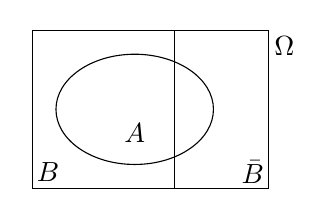
\begin{tikzpicture}
			\draw (0,0) rectangle (3,2);
			\draw (1.8,0) -- (1.8,2);
			\draw (1.3,1.0) ellipse (1.0cm and 0.7cm);
			\draw (0.2,0.2) node {$B$};
			\draw (2.8,0.2) node {$\bar{B}$};
			\draw (1.3,0.7) node {$A$};
			\draw (3.2,1.8) node {$\Omega$};
		\end{tikzpicture}
	\end{center}
	
    \begin{eqnarray*}
        P(A) = P(A \cap \Omega) &=& P(A \cap \sum\limits^n_{k=1} B_k)\\
        &=& P(\sum\limits_{k=1}^n(A \cup B_k))\\
                                &=& P((A \cap B) \cup (A \cap \bar{B}))\\
                                &=& P(A \cap B + A \cap \bar{B})\\
                                &=& P(A \cap B)+P(A \cap \bar{B})
    \end{eqnarray*}
    \begin{center}
		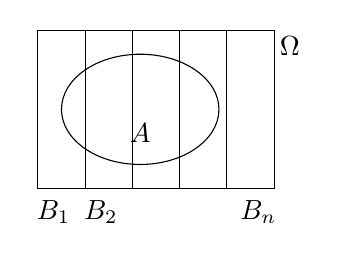
\begin{tikzpicture}
			\draw (0,0) rectangle (3,2);
			\draw (.6,0) -- (.6,2);
			\draw (1.2,0) -- (1.2,2);
			\draw (1.8,0) -- (1.8,2);
			\draw (2.4,0) -- (2.4,2);
			\draw (1.3,1.0) ellipse (1.0cm and 0.7cm);
			\draw (0.2,-.3) node {\(B_1\)};
			\draw (0.8,-.3) node {\(B_2\)};
			\draw (2.8,-.3) node {\(B_n\)};
			\draw (1.3,0.7) node {$A$};
			\draw (3.2,1.8) node {$\Omega$};
		\end{tikzpicture}
	\end{center}
	\(P(A) = \sum_i P(A \cap B_i)\), wenn \(B_i \Omega\) partitioniert.

\end{shaded}
Für eine Beobachtung \(a_1, \dots, a_n\) eines HMM suchen wir \(P(A_1=a_1, \dots, A_n=a_n)\).
Die Schwierigkeit dabei ist, dass die Zustandsfolge unbekannt ist.
Der naiver Ansatz ist die disjunkte Zerlegung nach Zustandsfolge \(Z_1, \dots, Z_n\):
\[P(A_1=a_1, \dots, A_n=a_n) = \sum\limits_{z_1, \dots, z_n} P(A_1=a_1, \dots, A_n=a_n, Z_1=z_1, \dots, Z_n=z_n)\]
Da diese Summe aus \(|Z|^n\) Summanden besteht, ist dies jedoch ineffizient.
Die Laufzeit wäre: $O(|Z|^n\cdot n)$.

Mit dynamischer Programmiereung erhalten wir ein effizenters Verfahren dazu sei:
\begin{eqnarray}
	\alpha_t(j) &=& P(A_1=a_1, \dots, A_t=a_t,Z_t=j)\nonumber\\
				&=& \sum_i P(A_1=a_1, \dots, A_t=a_t, Z_{t-1}=i, Z_t=j)		\nonumber\\
				&=& \sum_i P(A_t=a_t\mid A_1=a_1, \dots, _{t-1}=a_{t-1}, Z_{t-1}=i,Z_t=j) \nonumber\\
				&& \cdot P(A_1=a_1, \dots, A_{t-1}=a_{t-1}, Z_{t-1}=i, Z_t=j)\nonumber\\
				&=& \sum_i P(A_t=a_t\mid Z_t=j) \cdot P(A_1=a_1,\dots, A_{t-1}=a_{t-1},Z_{t-1}=i,Z_t=j)\nonumber\\
				&=& \sum_i q_j(a_t) \cdot P(Z_t=j\mid Z_{t-1}=i) \cdot P(A_1=a_1, \cdots, A_{t-1}=a_{t-1}, Z_{t-1}=i)\nonumber\\
				&=& \sum_i q_j(a_t) \cdot p(i,j) \cdot \alpha_{t-1}(i)
				\label{eq:Forward_1}
\end{eqnarray}
Für t=1 gilt
\begin{equation}
	\alpha_1(j)=P(A_1=a_1, Z_1=j)=q_j(a_1)\cdot \pi_j
	\label{eq:Forward_2}
\end{equation}
Ferner gilt
\begin{eqnarray}
	P(A_1=a_1, \dots,A_n=a_n)	&=&\sum P(A_1=a_1, \dots, A_n=a_n, Z_n=j) \nonumber\\
								&=& \sum_j \alpha_n (j)
	\label{eq:Forward_3}
\end{eqnarray}
Mit den Ergebnissen aus (\ref{eq:Forward_1}), (\ref{eq:Forward_2}) und (\ref{eq:Forward_3}) lässt sich die Wahrscheinlichkeit der Beobachtung \(a_1, \dots, a_n\) berechnen.
Aufwand dazu \[\underbrace{\mathcal{O}(n\cdot|Z|)}_{\text{Tabellengröße}}\cdot\underbrace{\mathcal{O}(|Z|)}_{\text{Aufwand pro Zelle}}+\underbrace{\mathcal{O}(|Z|)}_{\text{Aufsummierung}}=\mathcal{O}(n\cdot|Z|^2)\]

\begin{figure}[htbp]
	\centering
	\begin{tikzpicture}[node distance=1.5cm]
		\node[state] (j)                 {j};
		\node[state] (i) [left=2cm of j]	{i};
        \node[state] (s1) [above=of i]	{};
		\node[state] (s2) [below=of i]	{};
		\node (at-1) [below =.5cm of s2] {\(a_{t-1}\)};
        \node (dots) [left=of at-1] {\(\dots\)};
        \node (a1) [left=of dots] {$a_1$};
		%\node[emission] (at) [below of=j] {\(a_t\)};
        \node[emission] (at) [right = 1.85cm of at-1] {\(a_t\)};
        \path[->]
			(s1) edge (j)
			(s2) edge (j)
			(i) edge [above] node {\(p(i,j)\)} (j)
			(j)	edge [right] node {\(q_j(a_t)\)} (at);
	\end{tikzpicture}
	\caption{Skizze des Forward-Algorithmus}
	\label{fig:Forward-Alg}
\end{figure}

\subsection{Backward-Algorithmus}
Gegeben eine Beobachtung \(a_1, \dots, a_n\), was ist der wahrscheinlichste Zustand in Schritt \(t\)?
Gesucht ist ein \(j\) mit \[P(Z_t=j\mid A_1=a_1, \dots, A_n=a_n)\] maximal.

Ansatz:
\begin{eqnarray*}
	&& P(A_1=a_1, \dots, A_n=a_n,Z_t=j)\\
	&=& P(A_{t+1}=a_{t+1}, \dots, A_n=a_n\mid A_1=a_1, \dots, A_t=a_t, Z_t=j)\\
	&&\cdot P(A_1=a_1, \dots, A_t=a_t,Z_t=j)\\
	&=& P(A_{t+1}=a_{t+1}, \dots, A_n=a_n\mid Z_t=j)\cdot P(A_1=a_1,\dots, A_t=a_t, Z_t=j)\\
	&=& \beta_t(j)\cdot\alpha_t(j)
\end{eqnarray*}
Ferner sei \(\beta_n(j)=1\) für alle \(j\).
Ähnlich wie in Forward-Algorithmus folgt:
\[\beta_t(j)=\sum_i p(j,i)\cdot q_i(a_{t+1}) \cdot \beta_{t+1}(i)\]

\begin{figure}[htbp]
	\centering
	\begin{tikzpicture}[node distance=1.5cm]
		\node[state] (j)				{\(j\)};
		\node[state] (s1)	[right of=j]	{};
		\node[state] (s2)	[above of=s1]	{};
		\node[state] (i)	[below of=s1]	{\(i\)};
		\node[emission] (at+1)	[below of=i]	{\(a_{t+1}\)};
		\node[emission] (at)	[left of=at+1]	{\(a_{t}\)};
		\node (...)				[right of=at+1]	{\(\dots\)};
		\node[emission]	(...)	[right of=...]	{\(a_n\)};
		\path[->] 
			(j) edge (s1)
			(j) edge (s2)
			(j) edge (i)
			(j) edge [right] node {\(p(j,i)\)} (i)
			(i)	edge [right] node {\(q_i(a_{t+1})\)} (at+1);
	\end{tikzpicture}
	\caption{Skizze des Backward-Algorithmuses}
\end{figure}

Die Laufzeit des Backward-Algorithmus liegt damit in
\[\underbrace{\mathcal{O}(n\cdot|Z|^2)}_{\alpha\text{-Tabelle}} + \underbrace{\mathcal{O}(n\cdot|Z|^2)}_{\beta\text{-Tabelle}} + \underbrace{\mathcal{O}(|Z|)}_{\text{Summe}}+\underbrace{\mathcal{O}(1)}_{\text{Zugriff auf }\alpha_t(j) \text{und }\beta_t(j)}=\mathcal{O}(n\cdot|Z|^2)\]


Die Wahrscheinlichkeit für den Zustand \(j\) im Schritt \(t\) ergibt sich aus
\begin{align*}
    P(Z_t=j\mid A_1=a_1, \dots, A_n=a_n) =&
    \frac{P(A_1=a_1,\ldots,A_n=a_n,Z_t=j)}{P(A_1=a_1,\ldots,A_n=a_n)}\\
=&\frac{\alpha_t(j)\cdot\beta_t(j)}{\sum_i \alpha_n(i)}
\end{align*}


\subsection{Posterior Decoding}
Wenn der Viterbi-Algorithmus viele unterschiedliche Pfade mit annähernd gleicher Wahrscheinlichkeit liefert, dann lässt sich die Wahl des wahrscheinlichsten Pfades nicht gut rechtfertigen.
Alternativ können wir mit dem Backward-Algorithmus die Folge der in jedem
Zeitpunkt $t$ wahrscheinlichsten Zustände
\[ \hat z_{t} = \arg_{j}\max P(Z_{t} = j \mid  A_{1} = a_{1}, \ldots, A_{n} = a_{n}) \]
bestimmen.
Diese muss jedoch keine zuverlässige Folge sein.

\begin{shaded}
\paragraph{Übung}
\label{par:ubung}

Es sollen codierende und nicht-codierende Abschnitte in DNA bestimmt werden.
Vorhanden sind:
\begin{itemize}
    \item einige codierende Sequenzen
    \item einige nicht-codierende Sequenzen
    \item große Menge an unbekannten Sequenzen
\end{itemize}
Gesucht ist ein Verfahren um codierende Regionen in DNA zu identifizieren,
gegeben eine DNA Sequenz.\\
Lösung:
\begin{itemize}
    \item Hidden-Markov-Model wie in BildX
    \item jeweils einen ML-Schäter für beide Zustandsmenge \{codierend,
        nicht-codierend\} (überwachtes Training)
    \item Übergangswahrscheinlichkeiten zwischen den Zustandsmengen \{codierend,
        nicht-codierend\} mittels unüberwachtem Training (Viterbi-Training oder
        Baum-Welch-Algorithmus)
    \item Backward-Algorithmus
        \begin{align*}
            P(Z_t \in \{a_c,c_c,g_c,t_c\} \mid  A_1=a_1,\ldots,A_n=a_n)=\\
            \sum\limits_{z\in a_c,c_c,g_c,t_c} P(Z_t=z\mid A_1=a_1,\ldots,A_n=a_n)
        \end{align*}
\end{itemize}
Wenn das Ergebnis größer als $\frac{1}{2}$ ist, ist es eine codierende Sequenz,
sonst uncodierend.
\end{shaded}

\begin{shaded}
\paragraph{Übung}
\label{par:ubung2}

Gegeben sei ein HMM.
In diesem werden die Zustände verdoppelt.
Wie muss sich die Länge der Trainigssequenz erhöhen, damit die gleiche Anzahl Zustandsübergänge vorhanden ist wie vorher.
Vereinfacht sein angenohmen das alle Zustandsübergänge die gleiche Wahrscheinlichkeiten besitzen.

Lösung:
\[\hat p(z,z') = \frac{n}{|z^2|}\]
Die Trainigssequenz muss 4-fach solang sein.
\end{shaded}

\subsection{Baum-Welch-Algorithmus}
Der Baum-Welch-Algorithmus wird benutzt, um die unbekannten Parameter eines Hidden Markov Models (HMM) zu finden.
Er nutzt dabei den Forward-Backward-Algorithmus zur Berechnung von Zwischenergebnissen, ist aber nicht mit diesem identisch.
Der Baum-Welch-Algorithmus ist ein erwartungsmaximierender Algorithmus.

Idee:
\begin{enumerate}
    \item HMM zufällig initialisieren
    \item Mit dem Backward-Algorithmus die Wahrscheinlickeit \[P(Z_{t} = j \mid  A_{1} = a_{1}, \ldots, A_{n} = a_{n})\]berechnen.
        Auf ähnliche Weise lassen sich \[P(Z_{t} = i, Z_{t+1} = j \mid A_{1} = a_{1}, \ldots, A_{n} = a_{n})\] berechnen.
        Damit lassen sich Erwartungswerte berechen für die Häufigkeit eines Zustandes, eines Zustandsübergangs oder einer Emission.
        Damit lassen sich Schätzer berechnen für die Parameter des HMM.
        Damit werden die Parameter des HMM geändert.
    \item Mehrfach iterieren, bis sich an den Parametern nichts mehr ändert, beste Lösung ausgeben (größte Wahrscheinlichkeit für Ausgabesequenz)
\end{enumerate}

\section{Lineare Regression}
\label{sec:lineare_regression}
Der Korrelationskoeffizent ist ein Maß für lineare Abhängigkeit zweier
Zufallsvariablen.
\begin{align*}
    \varrho = \frac{Cov(x,y)}{\sqrt{Var X Var Y}}
\end{align*}

Wir wollen eine abhängige Größe $Y$ als lineare Funktion in den Variablen
$f_1,\ldots, f_n$ (Features) darstellen.
\begin{align*}
    y=w_0+\sum\limits_{i=1}^n w_i f_i \qquad w\cdots \text{Gewichtsvektor}
\end{align*}
Mit $f_0=1$ gilt:
\begin{align*}
    y=\sum\limits_{i=0}^n w_i\cdot f_i= w \cdot f
\end{align*}
Für Trainingsdaten $y^{(i)}, f^{(i)}$ bestimmen wir$w$ so, dass der mittlere
quadratische Fehler
\begin{align*}
    \sum\limits_i {(w\cdot f^{(i)}-y^{(i)})}^2
\end{align*}
minimiert wird. Eine exakte Lösung ist möglich.

\section{Logistische Regression}
\label{sub:logistische_regression}

Für eine binäre Zielgröße $y$ wollen wir $P(Y=true\mid f)$ bestimmen. Da $w\cdot f$
jedoch beliebige Werte annehmen kann, betrachten wir den Quotienten (Odds)
\begin{align*}
    \frac{P(Y=true\mid f)}{1-P(Y=true\mid f)}
\end{align*}
Dieser nimmt Werte $\geq 0$ an. Ansatz daher:
\begin{align}
    \ln \frac{P(Y=true\mid f)}{1-P(Y=true\mid f)} = w\cdot f. \tag{1}\label{eq:one}
\end{align}
Damit folgt:
\begin{align*}
    \ln \frac{P(Y=true\mid f)}{1-P(Y=true\mid f)} &= w\cdot f\\
    \frac{P(Y=true\mid f)}{1-P(Y=true\mid f)} &= e^{w\cdot f}\\
    P(Y=true\mid f) &=e^{w\cdot f}\cdot (1-P(y=true\mid f))\\
    P(Y=true\mid f) &=e^{w\cdot f} - e^{w\cdot f}P(y=true\mid f)\\
    P(Y=true\mid f) + e^{w\cdot f}P(y=true\mid f)&=e^{w\cdot f} \\
    P(Y=true\mid f)\cdot (1+ e^{w\cdot f}) &=e^{w\cdot f} \\
    P(Y=true\mid f) &=\frac{e^{w\cdot f}}{1+ e^{w\cdot f}} \\
    P(Y=true\mid f) &=\frac{1}{1+ e^{-w\cdot f}} \tag{2}\label{eq:two}
\end{align*}
Die Funktion
\begin{align*}
x\mapsto \frac{1}{1+e^{-x}}
\end{align*}
heißt logistische Funktion.

Zur Klassifikation einer Beobachtung $f$ verwenden wir den Ansatz
\begin{align*}
    P(Y=true \mid f)> P(Y=false \mid f)
\end{align*}
und damit
\begin{align*}
    \frac{P(Y=true\mid f)}{1-P(Y=true\mid f)} > 1
\end{align*}
Mit \cref{eq:one} erhalten wir daraus
\begin{align*}
    w\cdot f>0
\end{align*}
\paragraph{Geometrische Interpretation:}
\label{par:geometrische_interpretation_}

$w\cdot f=0$ ist die Gleichung einer Hyperebene.

Zum lernen der Gewichte verwenden wir einen ML-Ansatz
\begin{align*}
    \hat w & = \arg\max_w \prod\limits_i P(Y=y^{(i)}\mid f^{(i)})\\
    \hat w & = \arg\max_w \sum\limits_i \log P(Y=y^{(i)}\mid f^{(i)})\\
    \hat w & = \arg\max_w \left(\sum\limits_i y^{(i)}\log P(Y=1\mid
        f^{(i)}) + \sum\limits_i (1-y^{(i)})\log P(Y=0\mid f^{(i)})\right)\\
    \hat w & = \arg\max_w \left(\sum\limits_i y^{(i)} \log
    \left(\frac{1}{1+e^{-wf}}\right)+
    \sum\limits_i (1-y^{(i)}) \log \left(\frac{e^{-wf}}{1+e^{-wf}}\right)\right)
\end{align*}
Um diese Gleichung zu lösen werden numerische Verfahren (konvexe Optimierung)
verwendet.

\section{Multinomiale logistische Regression}
\label{sec:multinomiale_logistische_regression}

Wir verallgemeinern die logistische Regression auf eine Menge von Klassen $C$.
Mit dem Spezialfall $C={true,false}$ haben wir ermittelt
\begin{align*}
    P(y=true\mid
    x)&=\frac{1}{1+e^{-wf}}=\frac{e^{wf}}{1+e^{wf}} &=\frac{1}{z}e^{wf}\\
    P(y=false\mid
    x)&=\frac{1}{1+e^{wf}} &=\frac{1}{z}e^{0}\\
\end{align*}
Mit $w_{true} = w,\; w_{false}=0$ lässt sich dies schreiben als
\begin{align*}
    P(Y=true\mid x)=\frac{1}{z}e^{w_{true}f},\; P(Y=false\mid
    x)=\frac{1}{z}e^{w_{false}f}.
\end{align*}
Ferner ist
\begin{align*}
    z=e^{w_{true}f}+e^{f_{false}f}
\end{align*}
ein Normierungsfaktor.
Ansatz für $c\in C$ daher
\begin{align*}
    P(c\mid x)=\frac{1}{z}e^{w_cf} \qquad \text{mit } z=\sum\limits_{c\in
        C}e^{w_cf}
\end{align*}
Zur Klassifikation verwenden wir
\begin{align*}
    \hat c =\argmax_{c\in C}(P(c\mid x))
\end{align*}

\subsubsection{Softmax-Funktion}
\label{ssub:softmax_funktion}

Die Softmax-Funktion ist
\begin{align*}
    \softmax(c,C)= \frac{e^{x_c}}{\sum\limits_{c\in C}e^{x_c}}
\end{align*}
\paragraph{Es gilt:}
\label{par:es_gilt_}
$0 < \softmax < 1$

Für $x_c \ll \max\{x_c\mid c\in C\}$ gilt $\softmax \approx 0$.

Für $x_c \ll x_{c'},$ für $c' \neq c$ ist $\softmax \approx 1$.

Für Werte $x_c$, die nicht zu dicht zusammen liegen gilt
\begin{align*}
\softmax(c,C)
\approx \begin{cases}1,& \text{ für }c=\argmax\{x_c\mid c\in C\}\\
0, & \text{ sonst }\end{cases}
\end{align*}
Die softmax Funktion ist differenzierbar.

Die Klassifikationswahrscheinlichkeiten lassen sich damit schreiben als
\begin{align*}
    P(c\mid x)=\softmax(c,\{w_c\cdot f \mid c\in C\})
    \tag{*}\label{eq:softmax}
\end{align*}

\begin{shaded}
\paragraph{Übung}
\label{par:ubungsm}
\begin{enumerate}
    \item Zeigen Sie, dass softmax eine Verallgemeinerung der logistischen
        Funktion ist.
    \begin{align*}
        \logistic(x)=\frac{1}{1+e^{-x}}=\frac{e^x}{1+e^x}=\frac{e^x}{e^x+e^0}=\frac{e^x}{\sum\limits_C
        e^{x_c}}
    \end{align*}
    \item Zeigen Sie, dass für jedes $K$ gilt: $\softmax(c,\{x_c\mid c\in
        C\})=\softmax(c,\{x_c+K\mid c\in C\})$.
        \begin{align*}
            \softmax(c,\{x_c\mid c\in C\}) &= \frac{e^{x_c+K}}{\sum\limits_{c\in
                    C}e^{x_c+K}} = \frac{e^{x_c}\cdot e^K}{\sum\limits_{c\in
                    C}e^{x_c}\cdot e^K}=\frac{e^{x_c}}{\sum\limits_{c\in
                    C}e^{x_c}}\\ 
            &= \softmax(c,\{x_c+K\mid c\in C\}) \tag{u2}\label{eq:u2}
        \end{align*}
\end{enumerate}
\end{shaded}
Wegen \cref{eq:u2} können wir in \cref{eq:softmax} daher ein Gewicht auf 0
setzen $w_{c'}=w_c-w_{c^*}$ für ein beliebiges $c^*\in C$. Damit sind nur noch
$|C|-1$ Gewichte zu lernen. Damit
\begin{align*}
    P(c\mid x)=\frac{e^{w_{c'}}f}{1+\sum\limits_{c\neq c^*}e^{x_c}f}.
\end{align*}

\begin{shaded}
\paragraph{Beispiel}
\label{par:beispielsw}
Erkennen von Objekten

Es sollen Bilder von Nägeln, Schrauben und Muttern korrekt klassifiziert werden.

Features:
\begin{align*}
    f_1(x)&=\begin{cases}1, & \text{ wenn in der Bildmitte ein helles Pixel }\\
        0, & \text{sonst} \end{cases}\\
    f_2(x)&=\frac{\text{Bildbreite}}{\text{Bildhöhe}}\\
    f_3(x)&=\text{Anzahl an Kanten}
\end{align*}
3 Gewichte für die 3 Features lernen und mit multinomialer Regression
klassifizieren.
\end{shaded}

\paragraph{Interpretation der logistischen Regression} als Maximum-Entropy-Model
\label{par:interpretation_der_logistischen_regression}

Bereits bekant: Entropie ist ein Maß für den Informationsgehalt, aber auch der
Unsicherheit.

Max-Entropie-Prinzip: Unter mehreren möglichen Verteilungen wählen wir jene mit
maximaler Entropie.

\begin{shaded}
\paragraph{Beispiel}
\label{par:beispielme}
Wir wissen, dass eine Zufallsvariable $X$ die Werte 1,2,3,4 annimmt. Ein
MaxEnt-Modell dazu ist die Gleichverteilung auf \{1,2,3,4\}. Wenn nun
zusätzlich bekannt ist, dass $P(X=1)=\frac{1}{2}$, erhalten wir als
MaxEnt-Modell \begin{tabular}[t]{cccc}
    1 & 2 & 3 & 4 \\\hline
    $\frac{1}{2}$ & $\frac{1}{6}$ & $\frac{1}{6}$ & $\frac{1}{6}$
\end{tabular}.
Sei ferner $P(X=3 \lor X=4)=\frac{1}{4}$ bekannt:
\begin{tabular}[t]{cccc}
    1 & 2 & 3 & 4 \\\hline
    $\frac{1}{2}$ & $\frac{1}{4}$ & $\frac{1}{8}$ & $\frac{1}{8}$
\end{tabular}.
\end{shaded}

Man kann zeigen, dass eine multinomiale logistische Regression eine Lösung des
Optimierungsproblems
\begin{align*}
\argmax_{p\in M} H(p)
\end{align*}
liefert. Deshalb wird die logistische
Regression auch als MaxEnt bezeichnet.

\section{Naive Bayes Klassifikator}
\label{sec:naive_bayes_klassifikator}

Ansatz:
\begin{align*}
    P(c,x)=\frac{P(c)P(x\mid c)}{P(x)}
\end{align*}
Klassifikationsregel:
\begin{align*}
    \hat c=\argmax\limits_{c\in C} P(c\mid x) \tag{*}\label{eq:klassbayes}
\end{align*}
Dabei ist $x=(x_1,x_2,\dots,x_n)$. Wenn die Zufallsvariablen $x_i$ bedingt
unabhängig gegben $c$ sind, gilt
\begin{align*}
    P(x\mid c)=P(x_1,\dots,x_n\mid c)=\prod_i P(x_i\mid c)
\end{align*}
so dass sich \cref{eq:klassbayes} vereinfacht zu
\begin{align*}
    \hat c= \argmax_{c\in C}p(c)\prod_i P(x_i\mid c)
\end{align*}
Die verschiedenen Varianten des Naive bayes unterscheiden sich in der
Modellierung von $P(x_i\mid c)$ (normalverteilt, multinomialverteilt,
Bernoulli, etc).
